\providecommand{\pgfsyspdfmark}[3]{}
\providecommand{\savepicturepage}[3]{}

\documentclass[11pt,letterpaper]{article}
\usepackage[lmargin=1in,rmargin=1in,tmargin=1in,bmargin=1in]{geometry}

% -------------------
% Packages
% -------------------
\usepackage{
	amsmath,			% Math Environments
	amssymb,			% Extended Symbols
	enumerate,		    % Enumerate Environments
	graphicx,			% Include Images
	lastpage,			% Reference Lastpage
	multicol,			% Use Multi-columns
	multirow,			% Use Multi-rows
	gensymb
}


% -------------------
% Font
% -------------------
\usepackage[T1]{fontenc}
\usepackage{charter}


% -------------------
% Commands
% -------------------

\newcommand{\prob}{\noindent\textbf{Problem. }}
\newcounter{problem}
\newcommand{\problem}[1]{
	\noindent \textbf{Problem #1. }%
}
\newcommand{\answer}{\noindent \textbf{Answer. }}
\newcommand{\pspace}{\par\vspace{\baselineskip}}
\newcommand{\ds}{\displaystyle}


% -------------------
% Header & Footer
% -------------------
\usepackage{fancyhdr}

\fancypagestyle{pages}{
	%Headers
	\fancyhead[L]{}
	\fancyhead[C]{}
	\fancyhead[R]{}
\renewcommand{\headrulewidth}{0pt}
	%Footers
	\fancyfoot[L]{}
	\fancyfoot[C]{}
	\fancyfoot[R]{}
\renewcommand{\footrulewidth}{0.0pt}
}
\headheight=0pt
\footskip=14pt

\pagestyle{pages}


% -------------------
% Content
% -------------------
\begin{document}
\noindent\textbf{\large Calculus II (MSF\_10010 / AM\_\_1080AH) \\ 2023 Spring \\ Answer Key to Selected Problems}

\bigskip

\problem{XIII-4} Let $f(x) = 2|x+1| - |x-2|$,
\begin{enumerate}[(a)]
    \item Derive reduced expressions for $f(x)$ under three scenarios: $x \le -1$, $-1 \le x \le 2$ and $x \ge 2$.
    \item Based on the above, graph $f(x)$ on a Cartesian plane with $x$-axis ranging from $x = -2$ to $x = 3$.
    \item Based on the above, evaluate
    \[\int_{-2}^3 f(x)~dx\]
\end{enumerate}

\smallskip

\answer
\begin{enumerate}[(a)]
    \item We evaluate $f(x)$ seperately under these three intervals
    \begin{enumerate}[(1)]
        \item When $x \le 1$, both $(x+1)$ and $(x-2)$ are non-positive, so $|x+1| = -(x+1)$ and $|x-2| = -(x-2)$, thus $f(x) = 2(-x-1)-(-x+2) = -x-4$
        \item When $-1 \le x \le 2$, only $(x-2)$ is non-positive, so $|x+1| = x+1$ and $|x-2| = -(x-2)$, thus $f(x) = 2(x+1)-(-x+2) = 3x$
        \item When $x \ge 2$, both $(x+1)$ and $(x-2)$ are non-negative, so $|x+1| = x+1$ and $|x-2| = x-2$, thus $f(x) = 2(x+1)-(x-2) = x+4$;
    \end{enumerate}
    \item As shown below, we can graph the function in a piecewise fashion with the expressions we just derived
    \begin{center}
        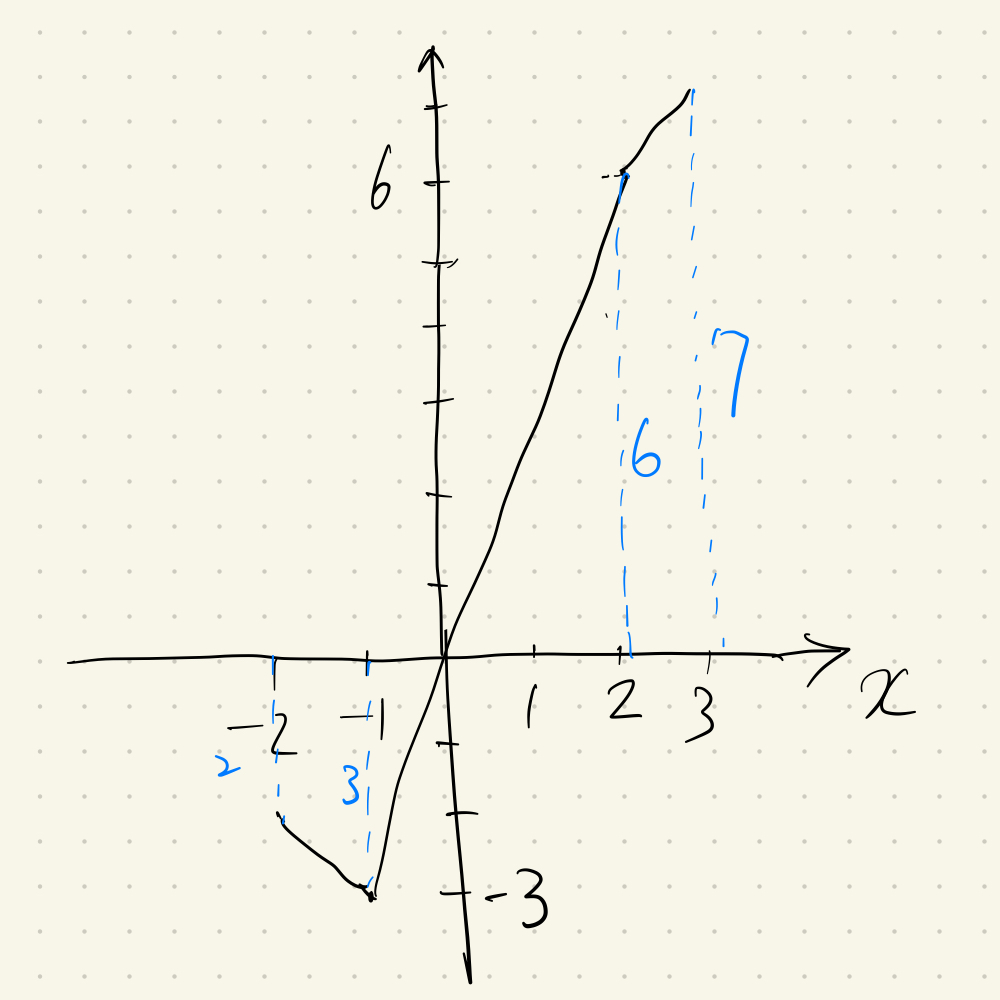
\includegraphics[width = 0.3\textwidth]{sol_abs.png}
    \end{center}
    \item The definite integral stands for the \textit{signed} area under curve between $x=-2$ and $x=3$.  The signed area between $x=0$ and $x=3$ is positive (since $f(x) \ge 0$ within this interval), and the area is the sum of a triangle and a trapezoid:
    \[\frac{2 \times 6}{2} + \frac{(6+7) \times 1}{2} = \frac{25}{2}\]
    The signed area between $x=-2$ and $x=0$ is negative (since $f(x) \le 0$ within this interval), and the area is also the sum of a triangle and a trapezoid:
    \[-\Big(\frac{1 \times 3}{2} + \frac{(2+3) \times 1}{2}\Big) = -4\]
    Therefore, the total signed area is
    \[\frac{25}{2}-4 = \frac{17}{2}\]
\end{enumerate}

\pagebreak

\problem{X-1} A solid is formed by revolving the area enclosed by $y = 2\sqrt{x}$, the $x$-axis and $x = 15$ around the $x$-axis.  Find the volume and surface area (including its round base perpendicular to the $x$-axis) of this solid. 

\smallskip

\answer The graph of the solid is as follows:
\begin{center}
    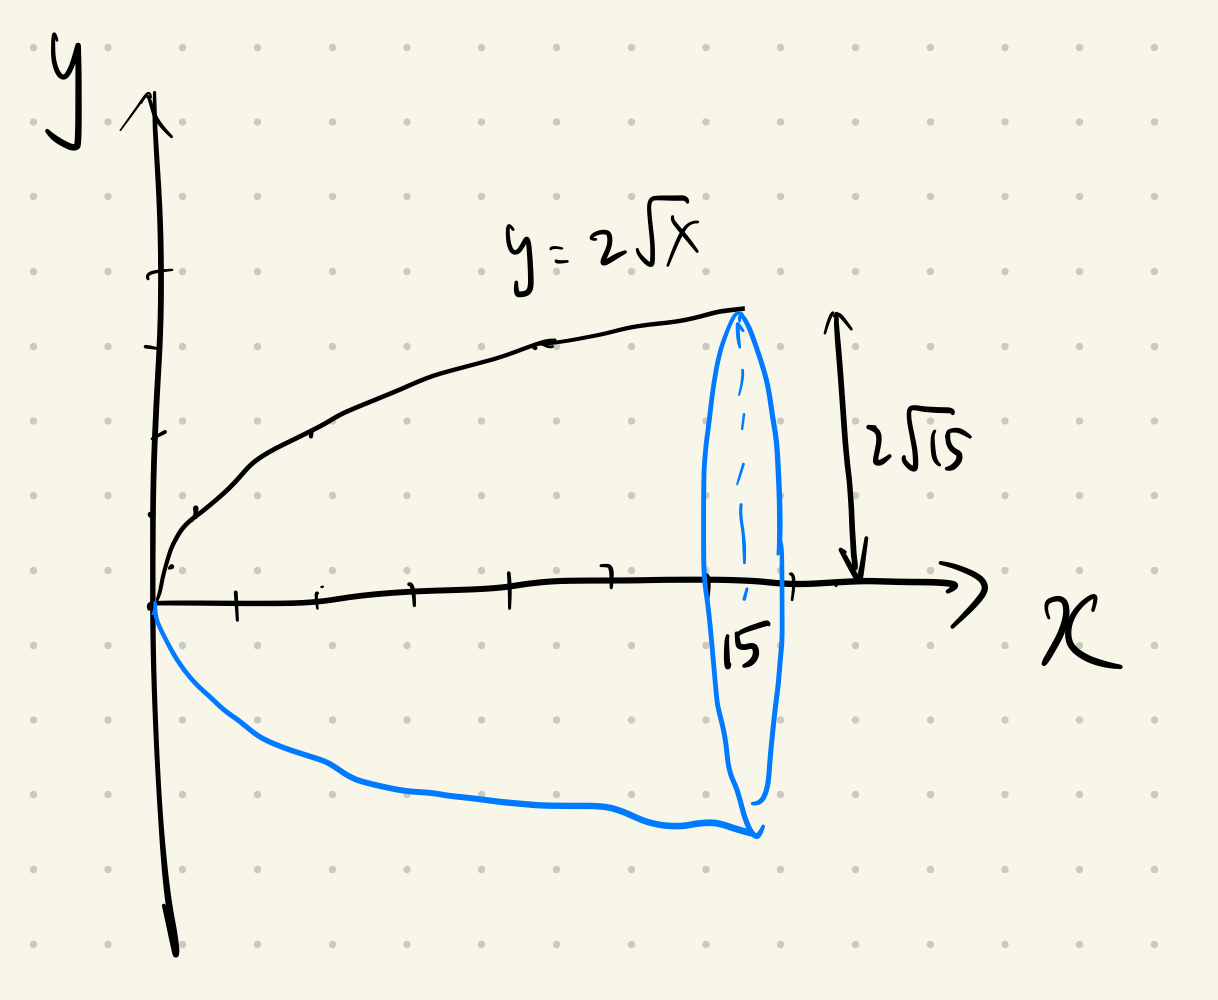
\includegraphics[width = 0.3\textwidth]{sol_rotate_x.png}
\end{center}
Using the method of disks, the volume can be calculated as 
\[V = \int_0^{15} \pi y^2~dx = \int_0^{15} \pi (2\sqrt{x})^2~dx = \int_0^{15} 4 \pi x~dx = 2 \pi x^2 \Big]_0^{15} = 2 \pi (225) = 450 \pi\]
The surface area can be split into the bell-shaped surface ($S_{Bell}$) and the bottom circle ($S_{Bot}$):
\begin{align*}
    S_{Bell} &= \int_0^{15} 2 \pi y~\sqrt{1+\big(\frac{dy}{dx}\big)^2}~dx \\
    &= \int_0^{15} 2 \pi (2\sqrt{x})~\sqrt{1 + \big(\frac{1}{\sqrt{x}}\big)^2}~dx\\
    &= \int_0^{15} 4 \pi \sqrt{x}~\sqrt{\frac{x+1}{x}}~dx\\
    &= \int_0^{15} 4 \pi \sqrt{x+1}~dx\\
    & = 4 \pi \cdot  \frac{2}{3}(x+1)^{3/2}\Big]_0^{15}\\
    &= 4 \pi \cdot (16^{3/2} - 1^{3/2}) = 4 \pi \cdot \frac{2}{3}(64-1) = 168 \pi
\end{align*}
Since the bottom is a circle of radius $2\sqrt{15}$
\[S_{Bot} = \pi (2\sqrt{15})^2 = 60 \pi\]
Therefore, the total surface area is 
\[S = S_{Bell} + S_{Bot} = 168 \pi + 60 \pi = 228 \pi\]

\pagebreak

\problem{X-3} A solid is formed by revolving the area enclosed by $y = \frac{1}{x}$, $y = 2$, the $x$- and $y$-axes and $x = 2$ around the $y$-axis.  Find the volume of this solid. 

\smallskip

\answer The shape of the solid is illustrated in the left panel of the following graph.  We can either use the method of disks cutting the solid along the $y$-axis or use the method of shells.  Since the shape rotating along the $y$-axis is irregular, both methods would require that we split the solid into two parts. 

\begin{center}
    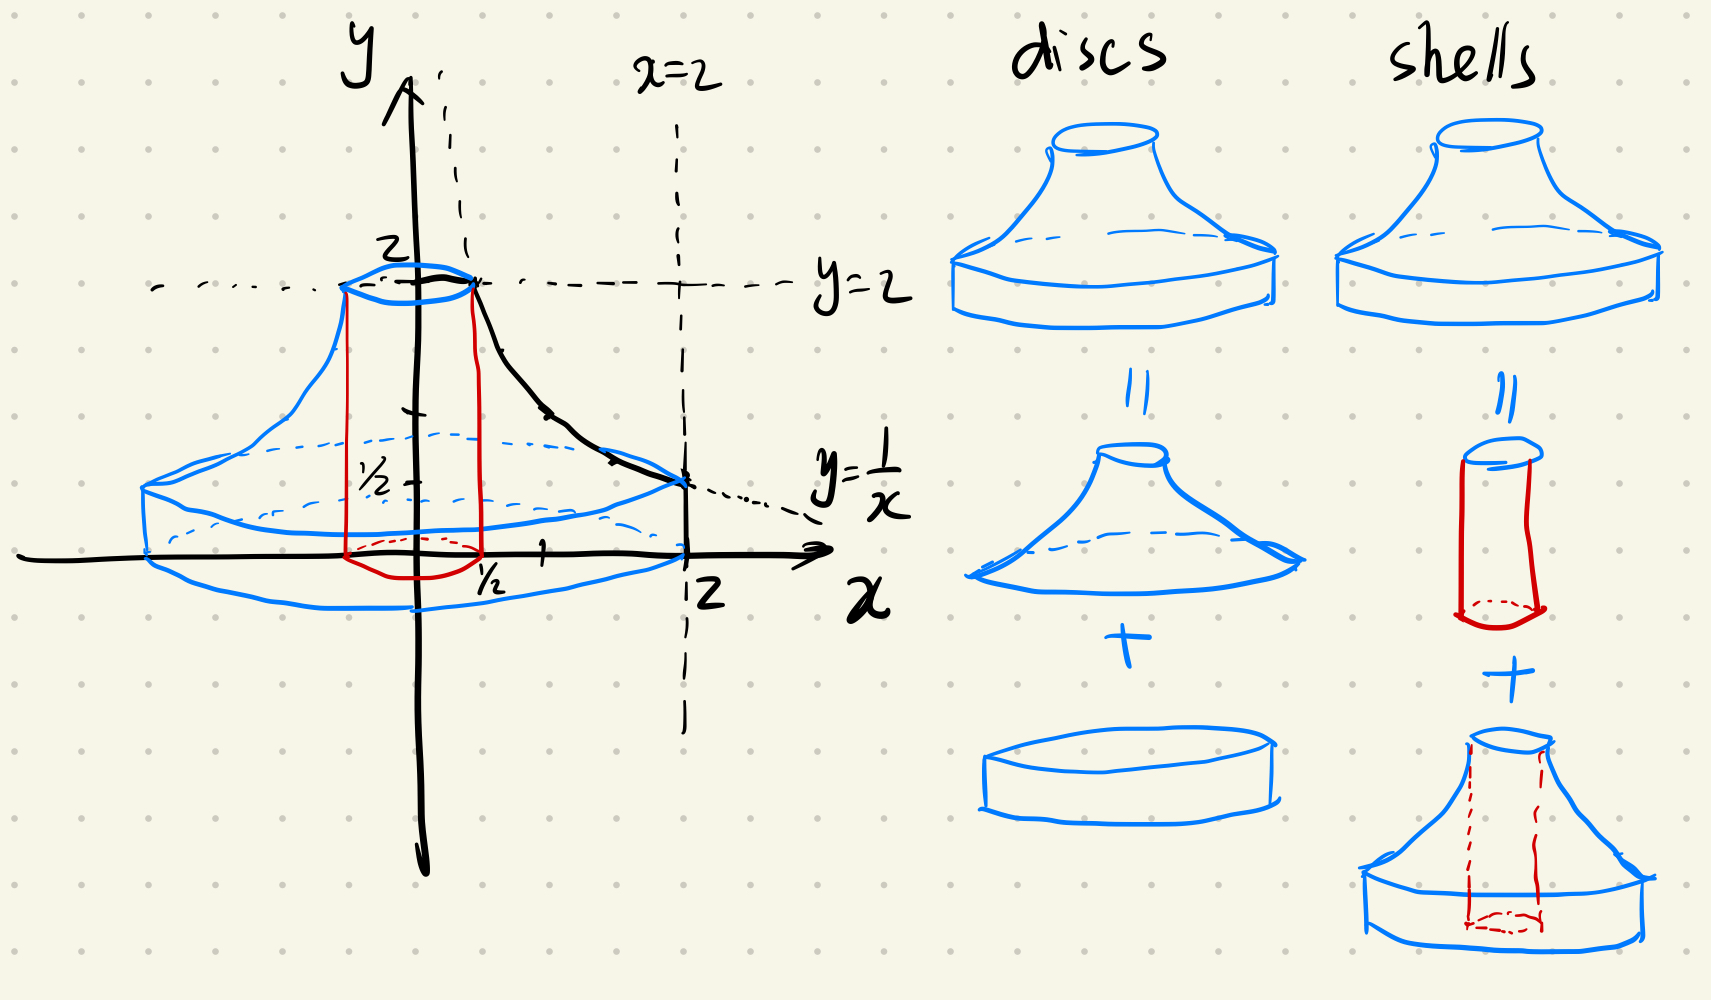
\includegraphics[width = 0.7\textwidth]{sol_rotate_y.png}
\end{center}

If we choose to use the method of disks, the solid can be split into a "volcano" part and "fat cylinder" part.  The volcano part is revolving $y=1/x$ from $y=1/2$ to $y=2$ around the $y$-axis.  Now we cut the solid along the $y$-axis to get sheets of thin disks of width $dy$.  If the $y$-coordinate of a disk is $y$, then its radius would be $1/y$ since we are rotating the curve of $y=1/x$.  Therefore, the volume of the disk would be $\pi (1/y)^2 \cdot dy$, and the volume of the volcano can be written as
\[V_{vol} = \int_{1/2}^2 \pi \Big(\frac{1}{y}\Big)^2~dy = -\frac{\pi}{y}\Big]_{1/2}^2 = -\frac{\pi}{2} - (-2\pi) = \frac{3}{2}\pi\]
The fat cylinder beneath the volcano is of radius $2$ and height $1/2$, so its volume is $V_{fat} = \pi \cdot 2^2 \cdot 1/2 = 2\pi$.  Finally, the total volume of the solid of revolution is 
\[V = V_{vol} + V_{fat} = \frac{3}{2}\pi + 2\pi = \frac{7}{2}\pi\]

Alternatively, we can use the method of shells, where we need to split the solid into a tall cylinder part and a hollow volcano part.  For the tall cylinder, its radius is $1/2$ and its height is $2$, so its volume is $V_{tall} = \pi \cdot (1/2)^2 \cdot 2 = \pi/2$.  For the hollow volcano part, if we slice it into concentric cylindrical shells of radius $x$ and width $dx$, then the height of the cylindrincal shells would be $1/x$ since we are rotating the curve of $y=1/x$.  Therefore, the volume of the shells would be $2\pi x \cdot (1/x) \cdot dx$.  Since the radius of the shells goes from $1/2$ to $2$, the volume of the hollow volcano can be found by the following integral:
\[V_{hol} = \int_{1/2}^2 2\pi x \cdot (1/x)~ dx = \int_{1/2}^2 2\pi~dx = 2\pi x\big]_{1/2}^2 = 3\pi\]
We can obtain the same result for the volume of the solid of revolution
\[V = V_{tall} + V_{hol} = \frac{1}{2}\pi + 3\pi = \frac{7}{2}\pi\]

\pagebreak

\problem{X-4} The \textit{Gabriel's horn} is constructed by revolving the curve of $y = \frac{1}{x}$ where $x \ge 1$ around the $x$-axis.  Show that the
volume of this solid of revolution is $\pi$.

\smallskip

\answer A solid constructed by revolving the curve of $y = 1/x$ from $x=1$ to $x=a$ around the $x$-axis has the following volume
\[\int_1^a \pi \Big(\frac{1}{x}\Big)^2~dx = \int_1^a \frac{\pi}{x^2}~dx \]
In this problem, the curve revolved has range $x \ge 1$, which corresponds to letting $a$ go to $\infty$.  Therefore, our desired volume is
\[\int_1^\infty \frac{\pi}{x^2}~dx = -\frac{\pi}{x}\Big]_1^\infty = \Big[\lim_{x \rightarrow \infty} \Big(-\frac{\pi}{x}\Big)\Big] - (-\pi) = 0 + \pi = \pi\]

\end{document}